\documentclass[margin=10pt]{standalone}
\usepackage{color,xcolor}
\usepackage{makecell}
\usepackage{tikz-qtree, tikz}
\usepackage{pgfplots}
\pgfplotsset{compat=1.11}
\usepackage[utf8]{inputenc}

\definecolor{myblue}{HTML}{0072BD}
\definecolor{mygreen}{HTML}{258F1B}
\definecolor{myred}{HTML}{C4000C}
\definecolor{darkgreen}{HTML}{0D330A}

\usetikzlibrary{decorations.pathreplacing,arrows,shapes,positioning,shadows,calc}
\usetikzlibrary{decorations, decorations.text,backgrounds}
% \tikzset{every picture/.style={font issue=\footnotesize},
%     font issue/.style={execute at begin picture={#1\selectfont}}
% }
\newcommand{\tick}{\tikz \draw[-,thick] (0,-0.2) -- +(0,0.2);}
\newcommand{\tickH}{\tikz \draw[-,thick] (-0.2,0) -- +(0.2,0);}
% \tikzset{
%   dot/.style={shape=circle,inner sep=0pt,minimum size=+1.6mm,label={#1}},
%   dot/.default=,
%   dot*/.style={dot={#1},fill=black},
%   dot*/.default=,
%   doto/.style={dot={#1},draw=red,solid,thick},
%   doto/.default=
%   shorten/.style={shorten >={#1},shorten <={#1}}
% }

\begin{document}
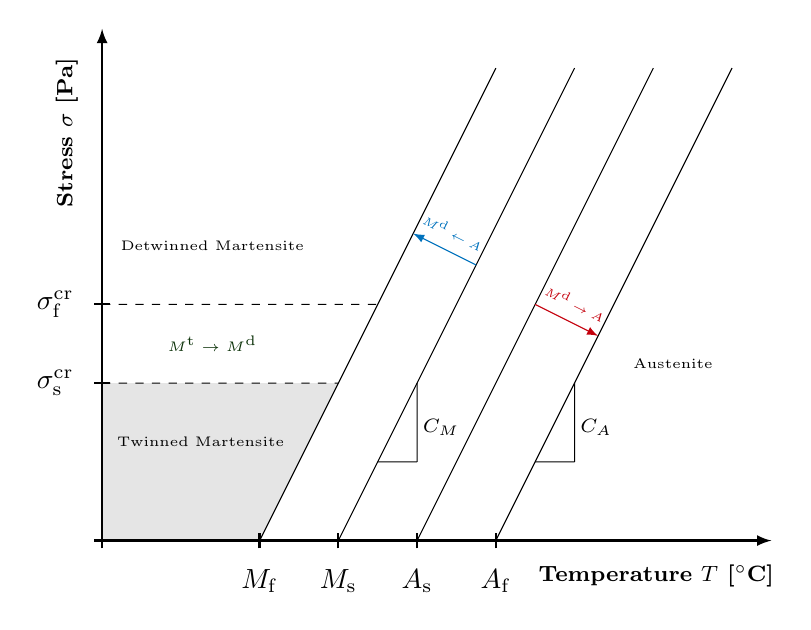
\begin{tikzpicture}
    % \draw[style=help lines,step=0.5cm] (0,0) grid (6.2,6.2);

    \draw[-latex,thick] (-0.1,0) -- (8.5,0) node[pos=0.83   ,below, yshift=-5]{\textbf{\footnotesize Temperature $T$ [$^\circ$C]}};
    \draw[-latex,thick] (0,-0.1) -- (0,6.5) node[pos=0.8,above,rotate=90, yshift=5] {\textbf{\footnotesize Stress $\sigma$ [Pa]}};

    % \foreach \x in {0,1,...,6} {
    %   \draw [thick](\x,-2pt) -- (\x,2pt) node[midway,below] {\x};
    %   \draw [thick](-2pt,\x) -- (2pt,\x) node[midway,left]  {\x};
    % }

    \coordinate (Mf) at (2,0);
    \node[label=below:$M_\mathrm{f}$] (Mftext) at (2,0) {\tick};
    \coordinate (Mf_) at ($(Mf)+(3,6)$);
    \coordinate (Ms) at (3,0);
    \node[label=below:$M_\mathrm{s}$] (Mstext) at (3,0) {\tick};
    \coordinate (Ms_) at ($(Ms)+(3,6)$) {};
    \coordinate (As) at (4,0);
    \node[label=below:$A_\mathrm{s}$] (Astext) at (4,0) {\tick};
    \coordinate (As_) at ($(As)+(3,6)$) {};
    \coordinate (Af) at (5,0);
    \node[label=below:$A_\mathrm{f}$] (Aftext) at (5,0) {\tick};
    \coordinate (Af_) at ($(Af)+(3,6)$) {};

    \coordinate (Cm) at ($(Ms)+(1,1)$) {};
    \node[label=right:{\scriptsize$C_M$},xshift=-5,yshift=12.5] (Cmtext) at (Cm) {};
    \coordinate (Cm'Ms) at (intersection of Cm--Ms|-Cm and Ms--Ms_);
    \coordinate (Cm'Ms_) at (intersection of Cm--Ms_-|Cm and Ms--Ms_);
    \path[-] (Cm) edge (Cm'Ms) edge (Cm'Ms_);

    \coordinate (Ca) at ($(Af)+(1,1)$) {};
    \node[label=right:{\scriptsize$C_A$},xshift=-5,yshift=12.5] (Catext) at (Ca) {};
    \coordinate (Ca'Af) at (intersection of Ca--Af|-Ca and Af--Af_);
    \coordinate (Ca'Af_) at (intersection of Ca--Af_-|Ca and Af--Af_);
    \path[-] (Ca) edge (Ca'Af) edge (Ca'Af_);

    \draw[-] (Mf) -- (Mf_);
    \draw[-] (Ms) -- (Ms_);
    \draw[-] (Af) -- (Af_);
    \draw[-] (As) -- (As_);

    \coordinate (ss) at (0,2);
    \node[label=left:$\sigma_\mathrm{s}^\mathrm{cr}$] (sstext) at (0,2) {\tickH};
    \coordinate (sf) at (0,3);
    \node[label=left:$\sigma_\mathrm{f}^\mathrm{cr}$] (sftext) at (0,3) {\tickH};

    \coordinate (ssline) at (intersection of ss--Mf|-ss and Mf--Mf_);
    \coordinate (sfline) at (intersection of sf--Mf|-sf and Mf--Mf_);
    \path[-, dashed] (ss) edge (ssline);
    \path[-, dashed] (sf) edge (sfline);

    \fill[fill=black,opacity=0.1] (0,0) -- (Mf) -- (ssline) -- (ss) -- cycle;
    \node[anchor=center] (twMtext) at (1.25,1.25) {\tiny Twinned Martensite};
    \node[anchor=center] (detwMtext) at (1.4,3.75) {\tiny Detwinned Martensite};
    \node[anchor=center] (twtodetw) at (1.4,2.5) {\color{darkgreen}\tiny $M^\mathrm{t}\rightarrow M^\mathrm{d}$};

    \node[anchor=center] (Atext) at (7.25,2.25) {\tiny Austenite};

    \coordinate (M2As) at ($(As)+(1.5,3)$);
    \draw[->,>=latex,color=myred] (M2As) -- node[above,sloped,scale=0.85,yshift=2] {\color{myred}\tiny $M^\mathrm{d}\rightarrow A$} ($(Af)!(M2As)!(Af_)$);

    \coordinate (A2Ms) at ($(Ms)+(1.75,3.5)$);
    \draw[->,>=latex,color=myblue] (A2Ms) -- node[above,sloped,scale=0.85,yshift=2] {\color{myblue}\tiny $M^\mathrm{d}\leftarrow A$} ($(Mf)!(A2Ms)!(Mf_)$);
\end{tikzpicture}
\end{document}
